\chapter{Research background}
\label{chap:Research background}
\lhead{\emph{Research background}}

\section{What is Autism?} 

To understand how an individual with Autism functions and reacts to computer-based instructions, it has to describe what Autism is and how their learning and social skills are affected. Autism is a developmental delay and disability that affects social interaction, social communication and social imagination; this is known as the triad of impairments~\cite{Reference6}. 

The first of the triad is social interaction; the person with Autism may not have an interest in a particular activity. It can be challenging for them to make friends with other individuals and individuals their age and typically have difficulties with maintaining eye contact; it may either be absent or indifferent. When a person with Autism does not initiate conversation or find it challenging to continue a conversation, they may also experience delayed language development and usually have a repetitive language or behaviour; this is the social communication impairment of the triad. The last of the triad is social imagination; individuals with Autism may not imagine what will happen, they often lack hindsight. Next, they may have limited creative skills or imaginative play; this affects their ability to keep or access information or memories related to personal experiences~\cite{Reference7}.

The triad of impairment in each person with ASD can differ based on the severity of the disability, individuals level of intelligence, personality traits, the presence of other disorders and if there has been the introduction of additional resources to improve the individuals disorder. Individuals with ASD may also experience sensory issues and be hypersensitive to smell, sound, taste, touch and visual stimulation. The world of a person with ASD can be challenging and confusing, to both the individual with Autism and those who are typically functioning. Individuals with ASD may rely on repetitive patterns and behaviours, become attached to particular physical objects, and only consume specific foods and drinks. People with ASD may lack responsiveness due to the triad of impairments, this is sometimes mistaken for being deaf or struggling with hearing ~\cite{Reference8}.

\section{Autism in education} 

In 2016, it was seen that 1 in 65 of the school-going population has a diagnosis of Autism~\cite{Reference9}.
It has been proven from existing research that children with Autism benefit greatly from education that is especially suited to their needs by educational professionals. The approaches must be widely available and ethical, so it does not cause distress to the person with Autism~\cite{Reference10}. The National Council for Special Education in Ireland details practical teaching strategies for students with Autism. Children with ASD can benefit from a combination of custom teach strategies, also known as an eclectic approach. This is when two or more strategies are combined for the student and their individual needs, this is a child-centred approach, this personalised approach is recommended for children with learning disabilities. Strategies listed include Lámh (language alternative for the mentally disabled), a manual signing language designed for individuals with ASD and other learning disabilities in Ireland. Another strategy that focuses on the individual teaching strategies for children with learning disabilities discussed is Teacch, originating from North Carolina and now adopted in Ireland, Teacch is a structured teaching approach for students with ASD~\cite{Reference11}. 

\section{What is Augmented Reality?}

Augmented Reality (AR) is described as the process of combining both real and computer generated assets that enhances the user's senses in vision, touch, hearing, taste and smell~\cite{Reference12}. It is described as an experience where parts of a user's physical world is combined through an immersive experience with computer-generated inputs; AR responds in real-time in the user's environment~\cite{Reference13}. AR can be dated back to 1901 and can be seen in science fiction movies; however, in 1990, Tomas Caudell described AR as a technology and how it was used to design Boeing's intricate aircraft system so workers could visualise the setup and therefore lowering human errors~\cite{Reference14}. 
% new line
 AR is under extended reality (XR) alongside virtual reality and mixed reality; AR differs from enhancing real-world views, not isolating the user from their environment, like virtual reality. Digital assets are superimposed, usually on a handheld smart device, to enhance the user's real-world environment. Pokemon Go, the mobile application released by the software company Niantic in July 2016, is an excellent real-life example of how AR works in real-time and in its environment; it uses GPS technology that inserts digital assets, the Pokemon characters, into the user's environment through a mobile device.
% new line 
 AR takes both real-world and a computer-generated world and is about how the two worlds interact with the both the real world and the digital world, it has a flexible immersion level, and the interface can be described as an out of screen experience for the users [X]. AR needs inputs and outputs; inputs from the user take form in movements, voice, controls and touch. These need to be high fidelity inputs to engage in an immersive experience. High fidelity inputs are accurate, precise and need to be comfortable for the user, while low fidelity inputs have errors, difficulties and are less precise and makes tasks increasingly difficult for the users~\cite{Reference15}.
 
 \section{How does Augmented Reality Work?}

AR incorporates computer-generated objects into a real-time environment for the user. To work it needs the following: 

\begin{itemize}
  \item Depth-sensing camera: Visual information must be recorded so computer-generated digital assets can be added to the application.
  \item Registration tools: Motion sensors and accelerometers are needed to define the space for superimposition of the digital assets into the real-world environment.
  \item Computer vision: A machine learning (ML) algorithm interprets the user's real-time environment and uses it as a reference point for the assets and their positioning. The pixels are used to recall similar-looking objects to give a high fidelity, precise and immersive experience. 
  \item Output device: This is the display where the user can experience the result; these displays can be devices such as smartphones and tablets that are widely accessible and affordable.
\end{itemize}

 \section{What are different types of Augmented Reality?}

AR enhances the user’s reality and can be carried out in different ways. 
A widely popular type of AR is Marker Based AR due to its availability and affordability. This type of AR needs an image or assets that acts as a marker for the AR technology making it more accurate and a better and more enjoyable experience for the user due to its immersive and high fidelity nature. 
\begin{itemize}
  \item Marker Based AR: This type of AR needs a distinct image or asset that acts as a marker for the technology. This type of AR is widely popular due to its availability and affordability. 
  \item Markerless AR: No marker is needed for this type of AR; you move the digital assets; an example is the international furniture company IKEA’s home remodelling application. This technology has no anchor needed for the real world.
  \item Projector based AR: This type of AR is complex and uses advanced technology. This type of technology is used in warehouses to simplify packing processes and training operations.
\end{itemize}

Augmented reality is widely used in businesses and industries to operate at their full potential and highest standard. It can be seen in industries from public safety to gaming, education, travel and equipment maintenance in both the medical and agricultural field.  

\Section {What is Artificial Intelligence?}

The definition of Artificial Intelligence is to enable computers and machines to interpret the perception, learning, problem-solving, and decision-making ability of, or as close to the human mind~\cite{Reference16}. AI is widely seen in everyday life; it can be challenging to understand due to the multiple terms, variations and interchangeable terms. AI can be linked with machine learning (ML), and deep learning (DL), speech recognition, natural language processing and can fall into either two categories of weak AI or strong AI~\cite{Reference17}.

 \section {What is difference between Artificial Intelligence, Deep Learning and Machine Learning?}
 
 \begin{itemize}
  \item Artificial Intelligence: Is the entirety of computing technology that resembles anything related to human intelligence.
  \item Machine Learning: This is a subset of AI that can learn by itself; the more data repeated to the technology helps it learn, recall and program itself for increased accuracy.
  \item Deep Learning: The models are based on deep neural networks with various layers; each layer refines the previous layer. The output layers are known as forwarding propagation and backpropagation that identify errors in calculations, and to  train the model for continuous accuracy.
\end{itemize}

 \section{What are different types of Augmented Reality?}
 
 AI can be broken into two different types, weak AI and strong AI~\cite{Reference18}.
 
  \begin{itemize}
  \item Weak AI: Described as Narrow AI or Artificial Narrow Intelligence (ANI), ANI is trained for specific tasks. Weak AI can be seen in most AI that exists. Narrow operates Apple's Siri and Amazon's Alexa.
  \item Strong AI: Artificial General Intelligence (AGI) replicates the autonomy of the human brain. AGI can choose the problems to solve without human intervention. 
\end{itemize}

AI applications and technology can be seen in everyday life; s common examples include speech to text, speech recognition, chat-bots in NPL, image recognition (computer vision or machine vision), automated stock trading and autopilot technology is only several applications using artificial intelligence functionality. 

As technology is ever evolving and changing meaning gaps in the market of technology and Autistic children are more apparent, there are numerous methods of technology such as machine learning, augmented reality, artificial intelligence, virtual reality, deep learning, gamification, convolution neural networks, and recurrent neural works have all been methods applied in the early diagnosis and intervention of a Child with ASD.Multiple research studies have been carried out in diagnosing and early intervention. However, there is a lack of research on the impact of augmented reality and artificial intelligence in the formal education of Autistic Children. This gap is significant because it gives scope for further research and development. The untapped potential in everyday technological devices as helpful tools could be huge for children with ASD. There are technological devices designed to function as tools in diagnosing and treating neurological disabilities. But, tiny amounts of technology for Autistic children and children with other developmental delays and learning disabilities and individualised technology for their additional needs.

\section{Facial expression and real time emotion computing}

Gamification plays a leading role when it comes to interaction among individuals with Autism and keeping them engaged and interactive, Paper one~\cite{Reference19} helps individuals with ASD understand other's emotions through computer-based instruction, gamification, real-time emotion computing and convolution neural networks (CNN). EmoTrain, the design concept and game engine, creates tasks that the user is expected to perform. Facial expressions and facial behaviour response skills of individuals with ASD are evaluated on the EmoTrain platform. This paper aims to improve individuals with ASD and their emotional intelligence and recognition through computer-based instructions and gamification. The papers main objectives are;

\begin{itemize}
    \item Using CNN to track facial expressions and emotions.
    \item Design EmoTrain, a real time emotion computing application to improve individuals with ASD emotional response.
    \item Understanding emotions in people 
    \texttt and improving an individual with 
    ASD and their response.
\end{itemize}

  \begin{figure}[h]
\centering
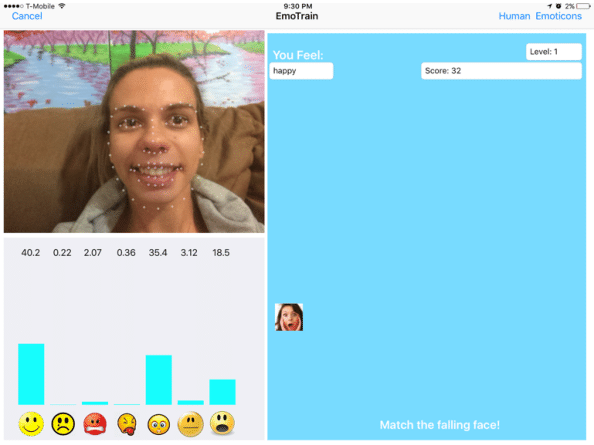
\includegraphics[width=0.5\textwidth]{IDD_LauraMartin_R00124705/Figures/emotrain.png}
\caption{EmoTrain prototype design}
\end{figure}

These objectives were tested by surveying after an evaluation study was carried out and nine subjects, aged 18 - 25 and diagnosed with ASD. Each participant received training with the EmoTrain platform two times a week, for two weeks and 20 minutes each session. 

\section{Augmented reality to improve elicit pretend play}
Children with Autism can lack in the ability to play with peers due to social and imaginative limitations, paper two~\cite{Reference20} helps children with Autism and who suffer from developmental delays with their symbolic thinking. The use of augmented reality (AR) is tested to improve elicit pretend play for Children with Autism. Areas that were focused on for improvement included individual differences, skill transfer, system usability and limitations of the proposed AR application was investigated for this paper. The design of an application for children with additional needs needs to be easy to navigate through that is why design guidelines for future AR systems for Children with ASD were also discussed for this paper. 

  This study aims to improve pretend play in children with ASC aged 4 - 7 through an interactive study that explores the possible potential of augmented reality (AR) technology taking into consideration the frequency, the duration and the relevance using the AR systems in comparison to non-computer assisted situations. 
  
  The main objectives of this paper are:
\begin{itemize}
    \item Improve pretend  play in children with Autism aged between 4 - 7 with AR implementation.  
    \item To investigate the individual differences, skill transfer, system usability, and proposed AR limitations.
\end{itemize}
  
  A  survey was conducted for both parents and the participants to collect qualitative data. The researchers considered the parents to supply more reliable data; each parent was asked to observe the participant playing and rate their engagement in cooperation, attentiveness and emotional response. Parents were also asked to complete a questionnaire; main questions included;
 
\begin{itemize}
    \item Which session do you think the participant enjoyed most?  
    \item One thing you like about the play?
    \item Are there other things you want to be on the screen?
    \item Which play is more fun?(with a friend/with the screen) and why?
\end{itemize}

Not all participants data was used for the analysis due to some participants being overwhelmed, and accurate data could not be collected. The mean frequency of pretend play recorded is higher in AR environments. Results included the mean frequency of constructive play was lower in non - AR conditions, the level of relational play, simple play and no play stays similar in both conditions, play duration was increased in AR conditions, engagement and cooperativeness are between average and high in both conditions.

\section{Autism and visual routines for effective teaching}
Children with Autism typically have visual routines introduced into their everyday life to improve social interactions and basic comprehensive understanding of everyday tasks, these visual routines act as instructions for the individual. In paper three~\cite{Reference21}  produces effective teaching, learning, and assisting aids for children with Autism and mild mental delays. The parent's voice is added to narrate the virtual 3D renderings that enhance the learning process, this comforts the child and gives them a sense of familiarity. The researchers used a mobile application that personalised AR lessons. The application supports functional reading, visual schedulers and speaking albums to learn in real-time environments.

This paper aims to implement assisting aids to automate functional reading, visual routines and picture exchange communications systems (PECS). These activities require hard copy materials. Information and communication technology (ICT) is used to make tedious activities more manageable and streamlined for parents/educators. The objectives and aims of this paper are:

\begin{itemize}
    \item To develop an e-Learning application called e-Sandhya is an accessible application for Children with ASD.  
    \item Streamline and automate functional reading, visual routines and PECS.
\end{itemize}

This paper had limitations in being validated as it failed to carry out a survey or collect any means of information for testing and validation.

\section {Autism through neuroimages and MRI data sets}

As there is increasing research into early diagnosis and intervention for an individual with Autism through neuroimages and MRI data sets. As an example of this work and research, paper four~\cite{Reference22} applies deep learning models, and image processing techniques are applied in clinical research to diagnose diseases. The researchers explain how it is challenging to diagnose ASD due to psychiatric symptoms. The contribution was investigating ASD using 14 different types of models, including convolutional neural networks (CNN) and recurrent neural networks (RNN) in more than 1000 MRI scans.
Paper five~\cite{Reference23} presents a systematic review of primary studies on the use of augmented reality (AR) to improve numerous skills of children and adolescents diagnosed with Autism spectrum disorders (ASD). The researchers planned and reviewed research questions, demographic information, learning skills and participant information was asked and analysed.

This paper aimed to introduce multiple deep learning models and CNN and RNN to diagnose the complex neurological disorders of ASD. To analyse neuroimages and MRIs to see recurring patterns in brain functionality in an individual with ASD. The outcome of this paper was to implement deep learning into the diagnostics of ASD in individuals through MRI scans and neuroimages.

Testing and data pre-processing were carried out; there were two studies and two MRI data sets for Autism. One from Yonsei University College of Medicine (YUM), and the second was a data set taken from the Autism Brain Imaging Data Exchange (ABIDE) web page, that gives access to many open-source MRIs for Autism research.

YUM carried out 84 studies with ABIDE carried out 1000+, the quality of the studies would be inaccurate and skewed as the same number of studies were not carried out. 

Both data sets could not record consistent information for comparison due to; data variability, sample size
and class labelling.


\section{Systematic review of research, demographic information and learning skills in Autistic Children}
Previous research has been carried out in relation to exploring the demographics and personal information through primary studies. In paper five  presented a systematic review of primary studies on the use of augmented reality (AR) to improve numerous skills of children and adolescents diagnosed with Autism spectrum disorders (ASD). The researchers planned and reviewed research questions, demographic information, learning skills and participant information was asked and analysed. The systematic review aims to address specific research questions regarding learning new skills, breaking restricted or repeat behaviours, AR technology, research design, data collection methods, intervention outcomes, and generalisation.
\paragraph{}
Sixteen research questions were asked, involving RQ and SRQ, analysing the questions. The top questions relevant to the study area are; Which settings are used in the primary studies?
\begin{enumerate}
    \item Classroom environment
    \item Community environment
    \item Controlled research environment
    \item School gymnasium
    \item Home environment
\end{enumerate}
Which data collection methods are used in the primary studies?
\begin{enumerate}
    \item Interview
    \item Focus group
    \item Programmatically
    \item Observation
    \item Questionnaire
\end{enumerate}

Areas of study focused on for research included; attention management, literacy, social communication, facial expressions and emotions. The results show that the frequency of access to the computer was higher than non-computer aided activities used for comparison. The addition of AR in maintaining a new skill varied from 2 to 9 weeks.
The participants targeted for the primary studies included typical, and individuals with ASD. 30 studies were recorded with 372 participants with a sample size of 1 to 92. All studies had an ASD individual.

\newpage
\section{Paper comparison table} 
Below is a detailed comparison of the papers discussed;
\begin{table} [h]
    \centering
\begin{tabular}{  m{2em} | m{7cm}| m{2cm} } 
\hline
Paper & Conclusion & XX   \\ 
\hline
1 & Tracks facial expressions and emotions to improve users emotional responses to other individuals.  \\ 
\hline
2 & Improves pretend play and symbolic thinking in individuals with ASD. The paper investigates individual differences, skills and possible limitations. \\ 
\hline
3 & Communications application to streamline and automate functional reading. \\ 
\hline
4 & Uses MRI data sets and neuroimages for early Autistic intervention and diagnosis through recurring data sets and MRI images. \\ 
\hline
5 & Detailed survey presenting a systematic review of augmented reality to improve numerous skills of children and adolescents with ASD. \\ 
\hline
\end{tabular}
\centering
\caption{Table of paper comparison}
    \label{tab:my_label}
\end{table}

\section{Conclusion}

Autism spectrum disorders have many layers to them and explanations, terms and disabilities  can be confusing to comprehend. Autism diagnosis is on the rise and it is becoming increasingly apparent that the personalised resources for those individuals diagnosed with the disability are limited or do not exist in today's market of applications and technology readily available. The applications that do exist for people with additional needs are designed to help with everyday social interactions, facial expression recognition and ways to improve it and fit into society while masking behaviours. This research paper is novel and differs from previous research material, the idea is to firstly get an understanding of the demographic, needs, struggles and limitations and the participants understanding of the technology available and understand their limitations when educating a child with Autism. This paper and idea are novel because of the proposed prototype design that is a markerless design and is an aid to non-verbal Autistic individuals and individuals with learning disabilities. The interviews conducted will give a better understanding of the demographic and market needs when it comes to using technology in the academic studies of children with ASD.



